\chapter{PROPOSED ALGORITHM AND DATA STRUCTURES}

\section{System Overview}

The \textit{Customer Journey Path Optimization} system will model user interactions as a directed weighted graph $G = (V, E)$, where each node $v \in V$ represents a discrete interaction state (e.g., \textit{Landing Page}, \textit{Search}, \textit{Product Page}, \textit{Cart}, \textit{Checkout}), and each directed edge $(u,v) \in E$ represents a user transition between states annotated with a transition probability $p(u,v) \in (0,1]$. The primary goal is to identify the most probable path from a designated source node $s$ to a target conversion node $t$.

Figure~\ref{fig:system_workflow} presents the end-to-end workflow process. The workflow process is organized into five sequential components: (1) data generation and preprocessing, (2) graph construction, (3) baseline path optimization using Dijkstra's algorithm, (4) optimized path search using probability-pruned Dijkstra, and (5) experimental evaluation and comparative analysis.

Two algorithms are proposed and compared throughout this chapter:
\begin{itemize}
    \item \textbf{Algorithm 1 --- Baseline Dijkstra on Log-Weights:} Standard Dijkstra's algorithm applied to the log-probability-transformed graph. Guarantees globally optimal paths in $O(|E|\log|V|)$ time.
    \item \textbf{Algorithm 2 --- Probability-Pruned Dijkstra:} Extension of Algorithm~1 with a pruning threshold $\tau$ that discards partial paths whose cumulative probability falls below $\tau$. Reduces expected runtime to $O(|E'|\log|V|)$, $|E'| \leq |E|$, with convergence to Algorithm~1 as $\tau \to 0$.
\end{itemize}

% ----------------------------------------------------------------
% FIGURE 1: System Workflow
% ----------------------------------------------------------------
\begin{figure}[h!]
\centering
\begin{tikzpicture}[
    node distance=0.6cm and 0.3cm,
    box/.style={rectangle, rounded corners=4pt, minimum width=2.6cm, minimum height=0.9cm,
                text centered, font=\small\bfseries, draw=black, thick},
    arrow/.style={-{Stealth[length=5pt]}, thick, color=arrowgray},
    label/.style={font=\scriptsize\itshape, text=gray}
]

% Step boxes
\node[box, fill=boxblue]  (s1) {Data Gen.};
\node[box, fill=boxblue, right=of s1]  (s2) {Graph Build};
\node[box, fill=boxorange, right=of s2] (s3) {Baseline Dijkstra};
\node[box, fill=boxgreen,  right=of s3] (s4) {Pruned Dijkstra};
\node[box, fill=boxgray,   right=of s4] (s5) {Evaluation};

% Arrows
\draw[arrow] (s1) -- (s2);
\draw[arrow] (s2) -- (s3);
\draw[arrow] (s3) -- (s4);
\draw[arrow] (s4) -- (s5);

% Sub-labels
\node[label, below=0.15cm of s1] {Synthetic \& Real};
\node[label, below=0.15cm of s2] {$G=(V,E),\; w(u,v)$};
\node[label, below=0.15cm of s3] {$O(|E|\log|V|)$};
\node[label, below=0.15cm of s4] {Threshold $\tau$};
\node[label, below=0.15cm of s5] {Metrics \& Trade-offs};

% Group bracket
\draw[decorate, decoration={brace, amplitude=6pt, mirror}, thick, color=nodeblue]
    ([xshift=-2pt, yshift=-1.1cm]s1.south west) -- ([xshift=2pt, yshift=-1.1cm]s5.south east)
    node[midway, below=8pt, font=\small\bfseries, color=nodeblue]
    {Customer Journey Path Optimization Workflow Process};
\end{tikzpicture}
\caption[System workflow overview]{Five-stage workflow process: data generation, graph construction, baseline Dijkstra, pruned Dijkstra, and experimental evaluation.}
\label{fig:system_workflow}
\end{figure}

\section{Problem Formulation}

\subsection{Graph Model and Inputs}

Customer interactions will be modeled as a directed graph $G = (V, E)$ with the following inputs:
\begin{itemize}
    \item $V$: the set of interaction states (nodes).
    \item $E \subseteq V \times V$: the set of directed transitions (edges).
    \item A transition probability function $p(u,v) \in (0,1]$ assigned to each edge $(u,v) \in E$.
    \item A designated source node $s \in V$ (e.g., Landing Page) and target node $t \in V$ (e.g., Checkout).
    \item A pruning threshold $\tau \in (0,1]$ used by the optimized algorithm to discard low-probability partial paths.
\end{itemize}

Figure~\ref{fig:journey_graph} illustrates a representative small customer journey graph to clarify the graph model.

% ----------------------------------------------------------------
% FIGURE 2: Example Customer Journey Graph
% ----------------------------------------------------------------
\begin{figure}[h!]
\centering
\begin{tikzpicture}[
    state/.style={circle, draw=black, thick, minimum size=1.15cm,
                  font=\small\bfseries, fill=boxblue},
    conv/.style={circle, draw=nodegreen!80!black, very thick, minimum size=1.15cm,
                 font=\small\bfseries, fill=boxgreen},
    src/.style={circle, draw=nodeorange!80!black, very thick, minimum size=1.15cm,
                font=\small\bfseries, fill=boxorange},
    epath/.style={-{Stealth[length=6pt]}, very thick, color=nodeblue},
    earrow/.style={-{Stealth[length=5pt]}, thick, color=black!40, dashed},
    elabel/.style={font=\scriptsize\itshape, fill=white, inner sep=1pt}
]
% ── Graph nodes (manual positioning for clarity) ──
\node[src]   (LP) at (0,0)     {LP};
\node[state] (SR) at (3.2,0)   {SR};
\node[state] (PP) at (6.4,1.4) {PP};
\node[state] (CT) at (6.4,-1.4){CT};
\node[conv]  (CK) at (9.6,1.4) {CK};

% ── Optimal path (solid blue) ──
\draw[epath] (LP) -- node[elabel,above]{$p=0.7$} (SR);
\draw[epath] (SR) -- node[elabel,above left]{$p=0.6$} (PP);
\draw[epath] (PP) -- node[elabel,above]{$p=0.8$} (CK);

% ── Alternative transitions (dashed) ──
\draw[earrow] (SR) -- node[elabel,below left]{$p=0.4$} (CT);
\draw[earrow] (CT) to[bend right=18] node[elabel,below right]{$p=0.3$} (CK);
\draw[earrow] (LP) to[bend right=30] node[elabel,below]{$p=0.3$} (CT);
\draw[earrow] (PP) -- node[elabel,right]{$p=0.2$} (CT);

% ── Legend box BELOW the graph, separated by white space ──
\node[draw=black!30, rounded corners=4pt, fill=white, inner sep=6pt,
      below=1.6cm of SR, xshift=1.8cm] (legbox) {%
  \begin{tabular}{@{}ll@{}}
    \tikz[baseline=-0.5ex]\draw[epath,shorten >=1pt] (0,0)--(0.55,0); &
      Optimal path $(s \!\to\! t)$\\[3pt]
    \tikz[baseline=-0.5ex]\draw[earrow,shorten >=1pt] (0,0)--(0.55,0); &
      Alternative transitions\\[3pt]
    \tikz[baseline=-0.5ex]\node[src,minimum size=0.38cm,inner sep=0pt,font=\tiny]{}; &
      Source $s$\ (LP = Landing Page)\\[3pt]
    \tikz[baseline=-0.5ex]\node[conv,minimum size=0.38cm,inner sep=0pt,font=\tiny]{}; &
      Target $t$\ (CK = Checkout)
  \end{tabular}
};
\end{tikzpicture}
\caption[Example customer journey graph]{Representative customer journey graph. Nodes are interaction states; LP = source $s$, CK = target $t$. Solid blue path LP$\to$SR$\to$PP$\to$CK is optimal ($\Pi^*=0.336$, log-cost$\approx1.091$); dashed edges are alternatives.}
\label{fig:journey_graph}
\end{figure}

\subsection{Probabilistic Path Objective and Outputs}

The graph in Figure~\ref{fig:journey_graph} shows five nodes connected by directed edges with transition probabilities. The optimal path LP$\to$SR$\to$PP$\to$CK (solid blue) achieves probability $0.7\times0.6\times0.8=0.336$. In log-space the edge weights are $-\log(0.7)\approx0.357$, $-\log(0.6)\approx0.511$, and $-\log(0.8)\approx0.223$, giving a total cost of approximately $1.091$ that Dijkstra's algorithm minimizes. Alternative lower-probability paths (dashed) are explored but not selected. Real graphs in this project will contain up to 50,000 nodes with sparse connectivity~\citep{bucklin2003clickstream}.

The goal is to find a path $P^* = (v_0 = s,\, v_1,\, \ldots,\, v_k = t)$ that maximizes the joint path probability~\citep{norris1998markov}:

\[
\max_{P} \prod_{(u,v) \in P} p(u,v)
\]

Directly multiplying many small probabilities causes numerical underflow~\citep{manning2008nlp}, a precision loss that renders long-path probability computations unreliable in floating-point arithmetic. To address this, each transition probability is transformed into an additive non-negative edge weight using the negative logarithm, a standard technique in probabilistic sequence modeling~\citep{viterbi1967error,rabiner1989hmm}:

\[
w(u,v) = -\log\bigl(p(u,v)\bigr)
\]

Since $p(u,v) \in (0,1]$, it follows that $w(u,v) \geq 0$ for all edges, satisfying the non-negativity requirement of Dijkstra's algorithm~\citep{cormen2009}. The maximization objective is then equivalently reformulated as a shortest-path minimization:

\[
\max \prod_{(u,v)\in P^*} p(u,v) \;\iff\; \min \sum_{(u,v)\in P^*} -\log\, p(u,v)
\]

If $p(u,v) = 0$ for any edge, that edge will be treated as infinite cost (non-traversable). If no path from $s$ to $t$ exists, the algorithm will report this correctly.

The system is expected to produce the following outputs:
\begin{itemize}
    \item The optimal or near-optimal path $P^* = (v_0 = s, v_1, \ldots, v_k = t)$.
    \item The path probability $\Pi^* = \prod_{(u,v)\in P^*} p(u,v)$.
    \item The log-transformed path cost $C^* = \sum_{(u,v)\in P^*} -\log\, p(u,v)$.
    \item Runtime and exploration metrics: execution time, peak memory usage, nodes explored, edges relaxed, and maximum priority queue size.
    \item Comparative performance results between the baseline and optimized algorithms across varying input sizes and threshold values.
\end{itemize}

\subsection{Constraints and Assumptions}

The following constraints and assumptions will govern the implementation:
\begin{itemize}
    \item Graph size may reach up to 50,000 nodes (hardware permitting).
    \item Graphs are assumed to be sparse ($|E| = O(|V|)$); an adjacency list will be used to maintain $O(|V|+|E|)$ space complexity~\citep{cormen2009}.
    \item Worst-case time complexity must remain polynomial.
    \item All transition probabilities are strictly positive; zero-probability edges are treated as non-traversable.
    \item A correct solution requires the baseline to return the globally optimal path, and the optimized algorithm to converge to the baseline when $\tau \to 0$.
\end{itemize}

\item The customer journey graph is allowed to contain directed cycles, reflecting realistic revisitation behavior (e.g., Browse $\rightarrow$ Product $\rightarrow$ Browse). No acyclicity assumption is imposed; correctness is preserved because the transformed edge weights remain non-negative, allowing Dijkstra's algorithm to operate correctly on cyclic graphs.

\section{Data Generation and Preprocessing}

\subsection{Synthetic Data Generation}

Synthetic customer journey graphs will serve as the primary dataset, providing full control over graph structure and enabling repeatable, scalable benchmarking. The generation methodology is grounded in the Erd\H{o}s--R\'{e}nyi random graph model~\citep{erdosrenyi1960}, which provides a theoretically principled basis for generating random directed graphs with predictable structural properties (connectivity and degree distribution) at a given size and density.

Graphs will be generated using the following procedure:

\begin{enumerate}
    \item Create $|V|$ nodes representing interaction states (e.g., Landing Page, Browse, Product Page, Cart, Checkout).
    \item For each node pair $(u,v)$, include a directed edge independently with probability $p_{\text{edge}} = \bar{d}/(|V|-1)$, where $\bar{d} \in \{2, 5, 10\}$ is the target average out-degree. This yields an expected total of $\bar{d} \cdot |V|$ edges, producing sparse graphs of varying density.
    \item Assign transition probabilities $p(u,v)$ to each edge under one of two distributions: (i) \textbf{uniform} $\mathcal{U}(0.1, 1.0]$, simulating balanced navigation behaviour; or (ii) \textbf{skewed power-law} with exponent $\alpha = 2$, where a small number of transitions carry high probability and the majority carry low probability, reflecting heterogeneous click patterns observed in real e-commerce data~\citep{bucklin2003clickstream}.
    \item Normalize outgoing probabilities for each node so that $\sum_v p(u,v) \leq 1$, ensuring a valid sub-stochastic transition system.
    \item Fix a designated source $s$ and target $t$, and guarantee at least one valid $s$-to-$t$ path using a depth-first path seeding step.
    \item Fix a random seed per configuration for full reproducibility across all 10 repeated runs.
\end{enumerate}

\noindent\textbf{Graph cycles.} Real customer journey data contains cycles: users frequently revisit states (e.g., \textit{Browse $\to$ Product $\to$ Browse $\to$ Cart}). The synthetic generator does \emph{not} enforce acyclicity; cycles arise naturally from the random edge-sampling procedure, mirroring real navigation behaviour. As established in Chapter~2, Dijkstra's algorithm remains fully correct on these cyclic graphs because the log-probability transformation $w(u,v) = -\log\,p(u,v) \geq 0$ guarantees non-negative edge weights~\citep{cormen2009}. Each cycle traversal adds strictly positive cost, so no node is ever re-finalized. No cycle detection or DAG preprocessing is required.

Synthetic generation is preferred as the primary substrate because it enables independent control of $|V|$, $|E|$, and the probability distribution---variables that cannot be decoupled in observational data. Input sizes will span three scales: small ($|V| \approx 1{,}000$), medium ($|V| \in [5{,}000,\; 10{,}000]$), and large ($|V|$ up to 50,000 nodes). Real-world datasets (RetailRocket~\citep{retailrocket2015}, UCI E-Commerce Clickstream~\citep{uci2008eshop}) are used as secondary validation benchmarks.

In addition to the Erd\H{o}s--R\'enyi-style sparse random generator, a second \emph{layered/stage-based graph generator} will be included to better reflect realistic customer-journey structure. In this generator, nodes are partitioned into ordered behavioral stages such as Awareness, Consideration, Intent, and Conversion, and transitions are sampled primarily between adjacent or near-adjacent stages, with limited backward or within-stage links to preserve realistic revisitation behavior. This provides a more domain-representative graph topology while retaining controlled variation in size, density, and probability distribution.

Using both generators strengthens the evaluation design: the random generator tests algorithmic behavior on generic sparse graphs, while the layered generator evaluates performance on more realistic customer-journey graphs.

\subsection{Real-World Clickstream Data}

Two real-world clickstream datasets will be used for secondary validation:

\begin{itemize}
    \item \textbf{RetailRocket E-Commerce Dataset}~\citep{retailrocket2015}: A publicly available Kaggle dataset containing approximately 2.7 million clickstream events across 235,000 items, collected from a real e-commerce platform. Sessions are extracted and state-transition sequences constructed from \texttt{view}, \texttt{addtocart}, and \texttt{transaction} events.
    \item \textbf{UCI E-Commerce Clickstream Dataset}~\citep{uci2008eshop}: A dataset from the UCI Machine Learning Repository containing approximately 165,000 user sessions for an online clothing store, with page-level interaction sequences suitable for constructing a small-to-medium navigation graph (${\sim}12$ states, ${\sim}40$ transitions).
\end{itemize}

Raw session data will be preprocessed by grouping interactions by \texttt{session\_id} and computing transition frequencies. Transition probabilities will be estimated using the maximum likelihood estimator~\citep{norris1998markov}:

\[
\hat{p}(u,v) = \frac{\text{count}(u \to v)}{\displaystyle\sum_{w:\,(u,w)\in E} \text{count}(u \to w)}
\]

\subsection{Sample Data Structure}

Table~\ref{table:data_structure} summarizes the structure of the enhanced synthetic dataset used to simulate real-world e-commerce behaviour.

\begin{table}[h!]
\centering
\begin{tabular}{@{}ll@{}}
\toprule
\textbf{Feature} & \textbf{Description} \\
\midrule
\texttt{session\_id} & Unique identifier for each user session. \\
\texttt{step} & Sequential step number within the session (1-indexed). \\
\texttt{timestamp} & UTC date and time of the interaction event. \\
\texttt{location} & Simulated user location (e.g., Thailand, Other). \\
\texttt{source} & Current interaction state (origin node $u$). \\
\texttt{target} & Next interaction state (destination node $v$). \\
\texttt{category} & Product category if applicable (e.g., Electronics, Clothing). \\
\texttt{price} & Numerical price of the viewed product (USD). \\
\texttt{is\_high\_price} & Binary flag: 1 if price exceeds \$200, 0 otherwise. \\
\bottomrule
\end{tabular}
\caption[Clickstream dataset schema]{Schema of the synthetic clickstream dataset. Each row is one state transition; \texttt{source}--\texttt{target} pairs are aggregated to estimate edge transition probabilities $p(u,v)$.}
\label{table:data_structure}
\end{table}

\section{Graph Construction}

The directed weighted graph will be constructed from preprocessed session data using an \textbf{adjacency list} representation. Each node $u$ maps to a list of $(v,\; w(u,v))$ pairs, where $w(u,v) = -\log(\hat{p}(u,v))$. This provides $O(|V|+|E|)$ space complexity and efficient $O(\deg(u))$ neighbour iteration~\citep{cormen2009}. An adjacency list is chosen over an adjacency matrix because customer journey graphs are sparse ($|E| \ll |V|^2$): most interaction states transition to only a small number of next states, so a matrix representation would waste $O(|V|^2)$ space storing mostly zeros.

\section{Algorithmic Approaches}

\subsection{Baseline Algorithm: Dijkstra's Shortest Path (Greedy Paradigm)}

The baseline applies Dijkstra's algorithm~\citep{dijkstra1959} to the log-transformed graph. Dijkstra's algorithm is a \textbf{greedy graph algorithm}~\citep{cormen2009}: at each step it irrevocably selects the unvisited node with the smallest accumulated cost, never reconsidering this choice. This greedy selection is valid precisely because all edge weights are non-negative, guaranteeing that the first time a node is extracted from the priority queue its distance is already optimal. A \textbf{binary min-heap} serves as the priority queue, achieving $O(\log|V|)$ extract-min and insert~\citep{cormen2009}. Since Python's \texttt{heapq} module does not support decrease-key, \textbf{lazy insertion} is used: when a shorter path to a node is found, a new entry is pushed and stale entries skipped when popped.

\begin{tcolorbox}[title=Algorithm 1: Dijkstra on Transformed Probabilities \citep{dijkstra1959,cormen2009}]
\begin{lstlisting}
Initialize dist[v] = INF for all v in V
Initialize parent[v] = NIL for all v in V
dist[s] = 0
Insert (0, s) into priority queue Q

While Q is not empty:
    (d, u) = Extract-Min(Q)
    if u == t: break          // optimal path reached
    if d > dist[u]: continue  // stale entry (lazy deletion)
    For each edge (u, v) with weight w = -log(p(u,v)):
        new_dist = dist[u] + w
        If new_dist < dist[v]:
            dist[v] = new_dist
            parent[v] = u
            Insert (new_dist, v) into Q

Return dist[t], exp(-dist[t]), ReconstructPath(parent, s, t)
\end{lstlisting}
\end{tcolorbox}

\noindent\textbf{Time complexity:} $O(|E| \log |V|)$ with a binary heap~\citep{cormen2009}. A Fibonacci heap would give $O(|E| + |V|\log|V|)$~\citep{fredman1987fibonacci}, but binary heaps are used here for practical efficiency.\\
\textbf{Space complexity:} $O(|V| + |E|)$.\\
\textbf{Optimality:} Guaranteed, since all $w(u,v) \geq 0$~\citep{dijkstra1959}.

\noindent\textbf{Worked Example: Dijkstra Step-by-Step.} Table~\ref{table:dijkstra_trace} traces Algorithm~1 on the five-node customer journey graph (Figure~\ref{fig:journey_graph}), illustrating how \texttt{dist[]} is updated at each extraction step.

\begin{table}[h!]
\centering
\begin{tabular}{@{}ccccccc@{}}
\toprule
\textbf{Step \#} & \textbf{Extract} & \textbf{LP} & \textbf{SR} & \textbf{PP} & \textbf{CK} & \textbf{AB} \\
\midrule
Init   & ---          & $0$    & $\infty$ & $\infty$ & $\infty$ & $\infty$ \\
1      & LP           & $0$    & $0.36$   & $\infty$ & $\infty$ & $\infty$ \\
2      & SR           & $0$    & $0.36$   & $0.87$   & $1.56$   & $\infty$ \\
3      & PP           & $0$    & $0.36$   & $0.87$   & $1.09$   & $2.48$ \\
4      & \textbf{CK}\checkmark & $0$ & $0.36$ & $0.87$ & \textbf{1.09} & $2.48$ \\
\bottomrule
\end{tabular}
\caption[Dijkstra dist{[}{]} trace on the example customer journey graph]{Dijkstra \texttt{dist[]} trace on the five-node graph, $s = \text{LP}$, $t = \text{CK}$. At step~4, CK is finalised with optimal log-cost $1.09$, corresponding to path LP$\to$SR$\to$PP$\to$CK with probability $\exp(-1.09) = 0.336 = 0.70 \times 0.60 \times 0.80$---a $1.60\times$ improvement over the shortcut LP$\to$SR$\to$CK ($p = 0.210$).}
\label{table:dijkstra_trace}
\end{table}

\begin{figure}[h!]
\centering
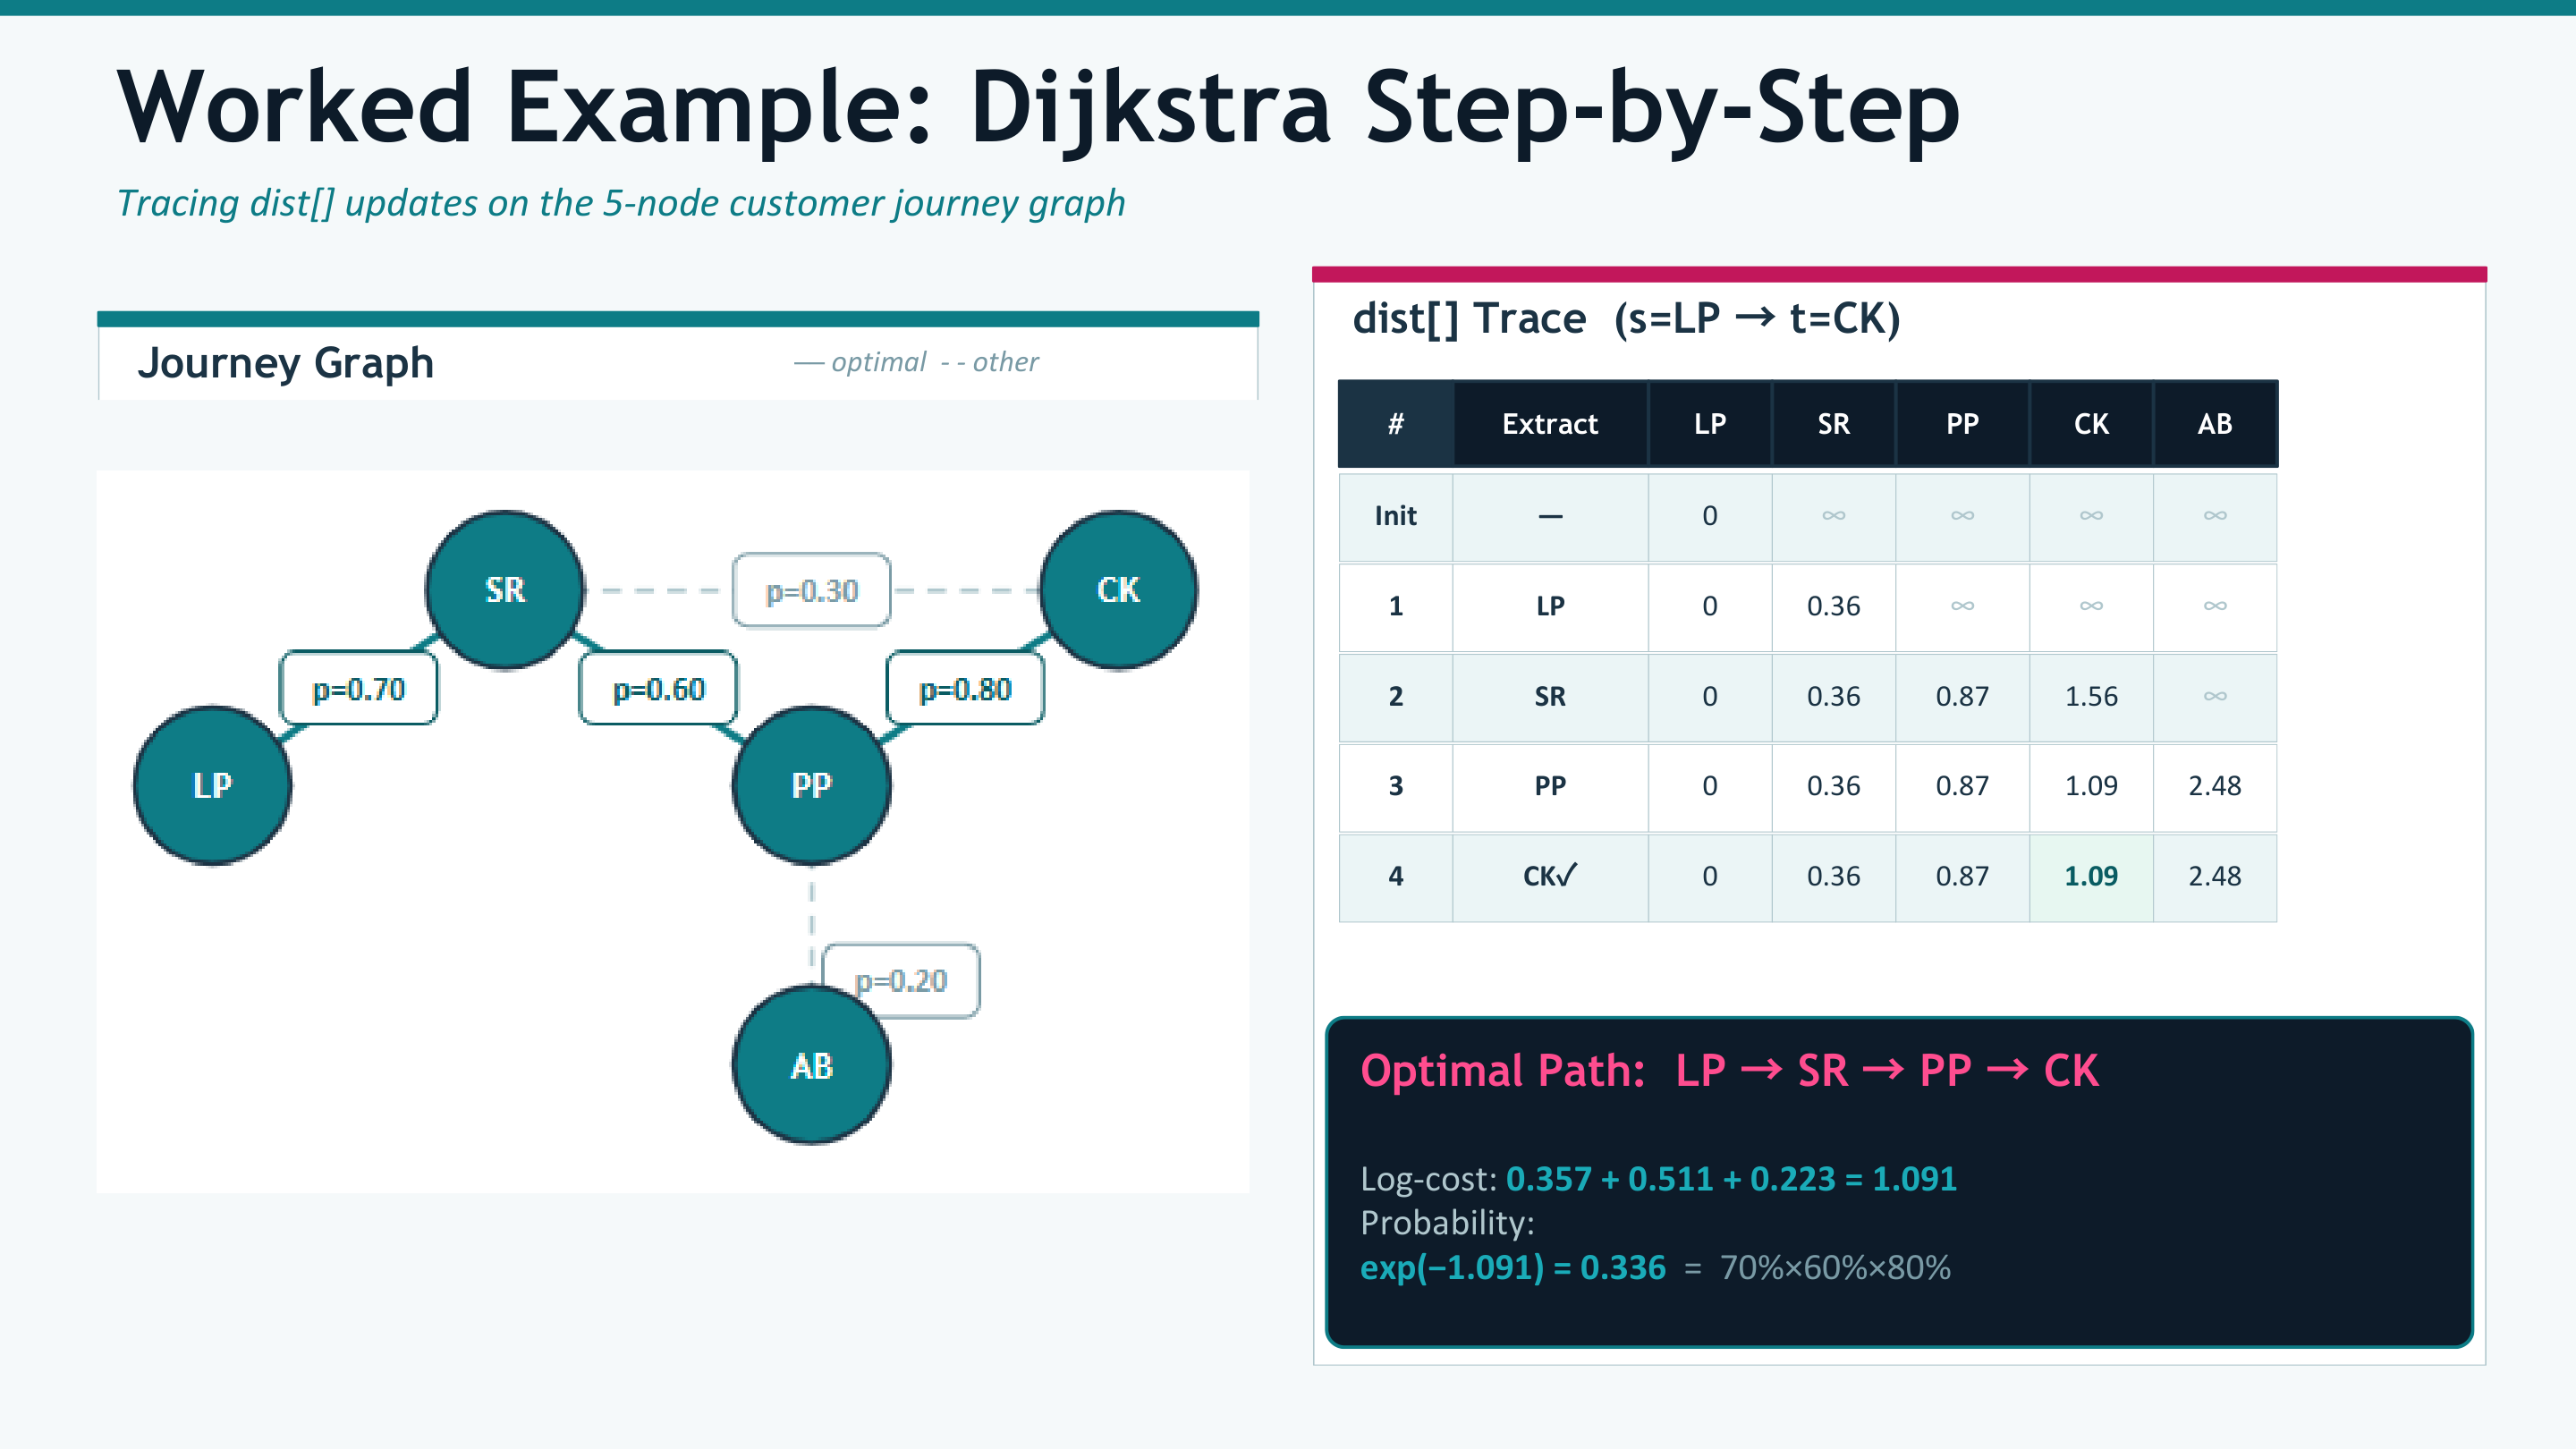
\includegraphics[width=0.92\textwidth]{worked_example}
\caption[Dijkstra step-by-step worked example]{Dijkstra step-by-step trace on the five-node customer journey graph ($s=\text{LP}$, $t=\text{CK}$). The left panel shows the graph with edge probabilities; the right panel tabulates the \texttt{dist[]} array after each node extraction. The optimal path LP$\to$SR$\to$PP$\to$CK is found with log-cost $1.091$ and probability $0.336$.}
\label{fig:worked_example}
\end{figure}

\subsection{Optimized Algorithm: Probability-Pruned Dijkstra (Approximation Technique)}

The proposed algorithm extends the baseline by introducing a \textbf{probability pruning threshold} $\tau \in (0, 1]$. This falls within the class of \textbf{approximation algorithms}~\citep{cormen2009}: it deliberately sacrifices worst-case optimality guarantees in exchange for improved practical runtime, while providing a controlled convergence guarantee ($\tau \to 0$ recovers exact optimality). The pruning is deterministic and parameter-controlled, distinguishing it from stochastic approximations such as Monte Carlo sampling or beam search. Any partial path whose cumulative probability falls below $\tau$ is pruned. In log-space, this is:

\[
\text{dist}[u] > -\log(\tau) = T
\]

\begin{tcolorbox}[title=Algorithm 2: Probability-Pruned Dijkstra]
\begin{lstlisting}
Initialize dist[v] = INF for all v in V
Initialize parent[v] = NIL for all v in V
dist[s] = 0
Insert (0, s) into priority queue Q
T = -log(tau)               // pruning threshold in log-space

While Q is not empty:
    (d, u) = Extract-Min(Q)
    if u == t: break
    if d > dist[u]: continue  // stale entry
    For each edge (u, v) with weight w = -log(p(u,v)):
        new_dist = dist[u] + w
        If new_dist > T: continue   // PRUNE: below probability tau
        If new_dist < dist[v]:
            dist[v] = new_dist
            parent[v] = u
            Insert (new_dist, v) into Q

Return dist[t], exp(-dist[t]), ReconstructPath(parent, s, t)
\end{lstlisting}
\end{tcolorbox}

\noindent\textbf{Worst-case time complexity:} $O(|E| \log |V|)$ (when $\tau \to 0$).\\
\textbf{Expected time complexity:} $O(|E'| \log |V|)$, $|E'| \leq |E|$.\\
\textbf{Space complexity:} $O(|V| + |E|)$.

\begin{figure}[h!]
\centering
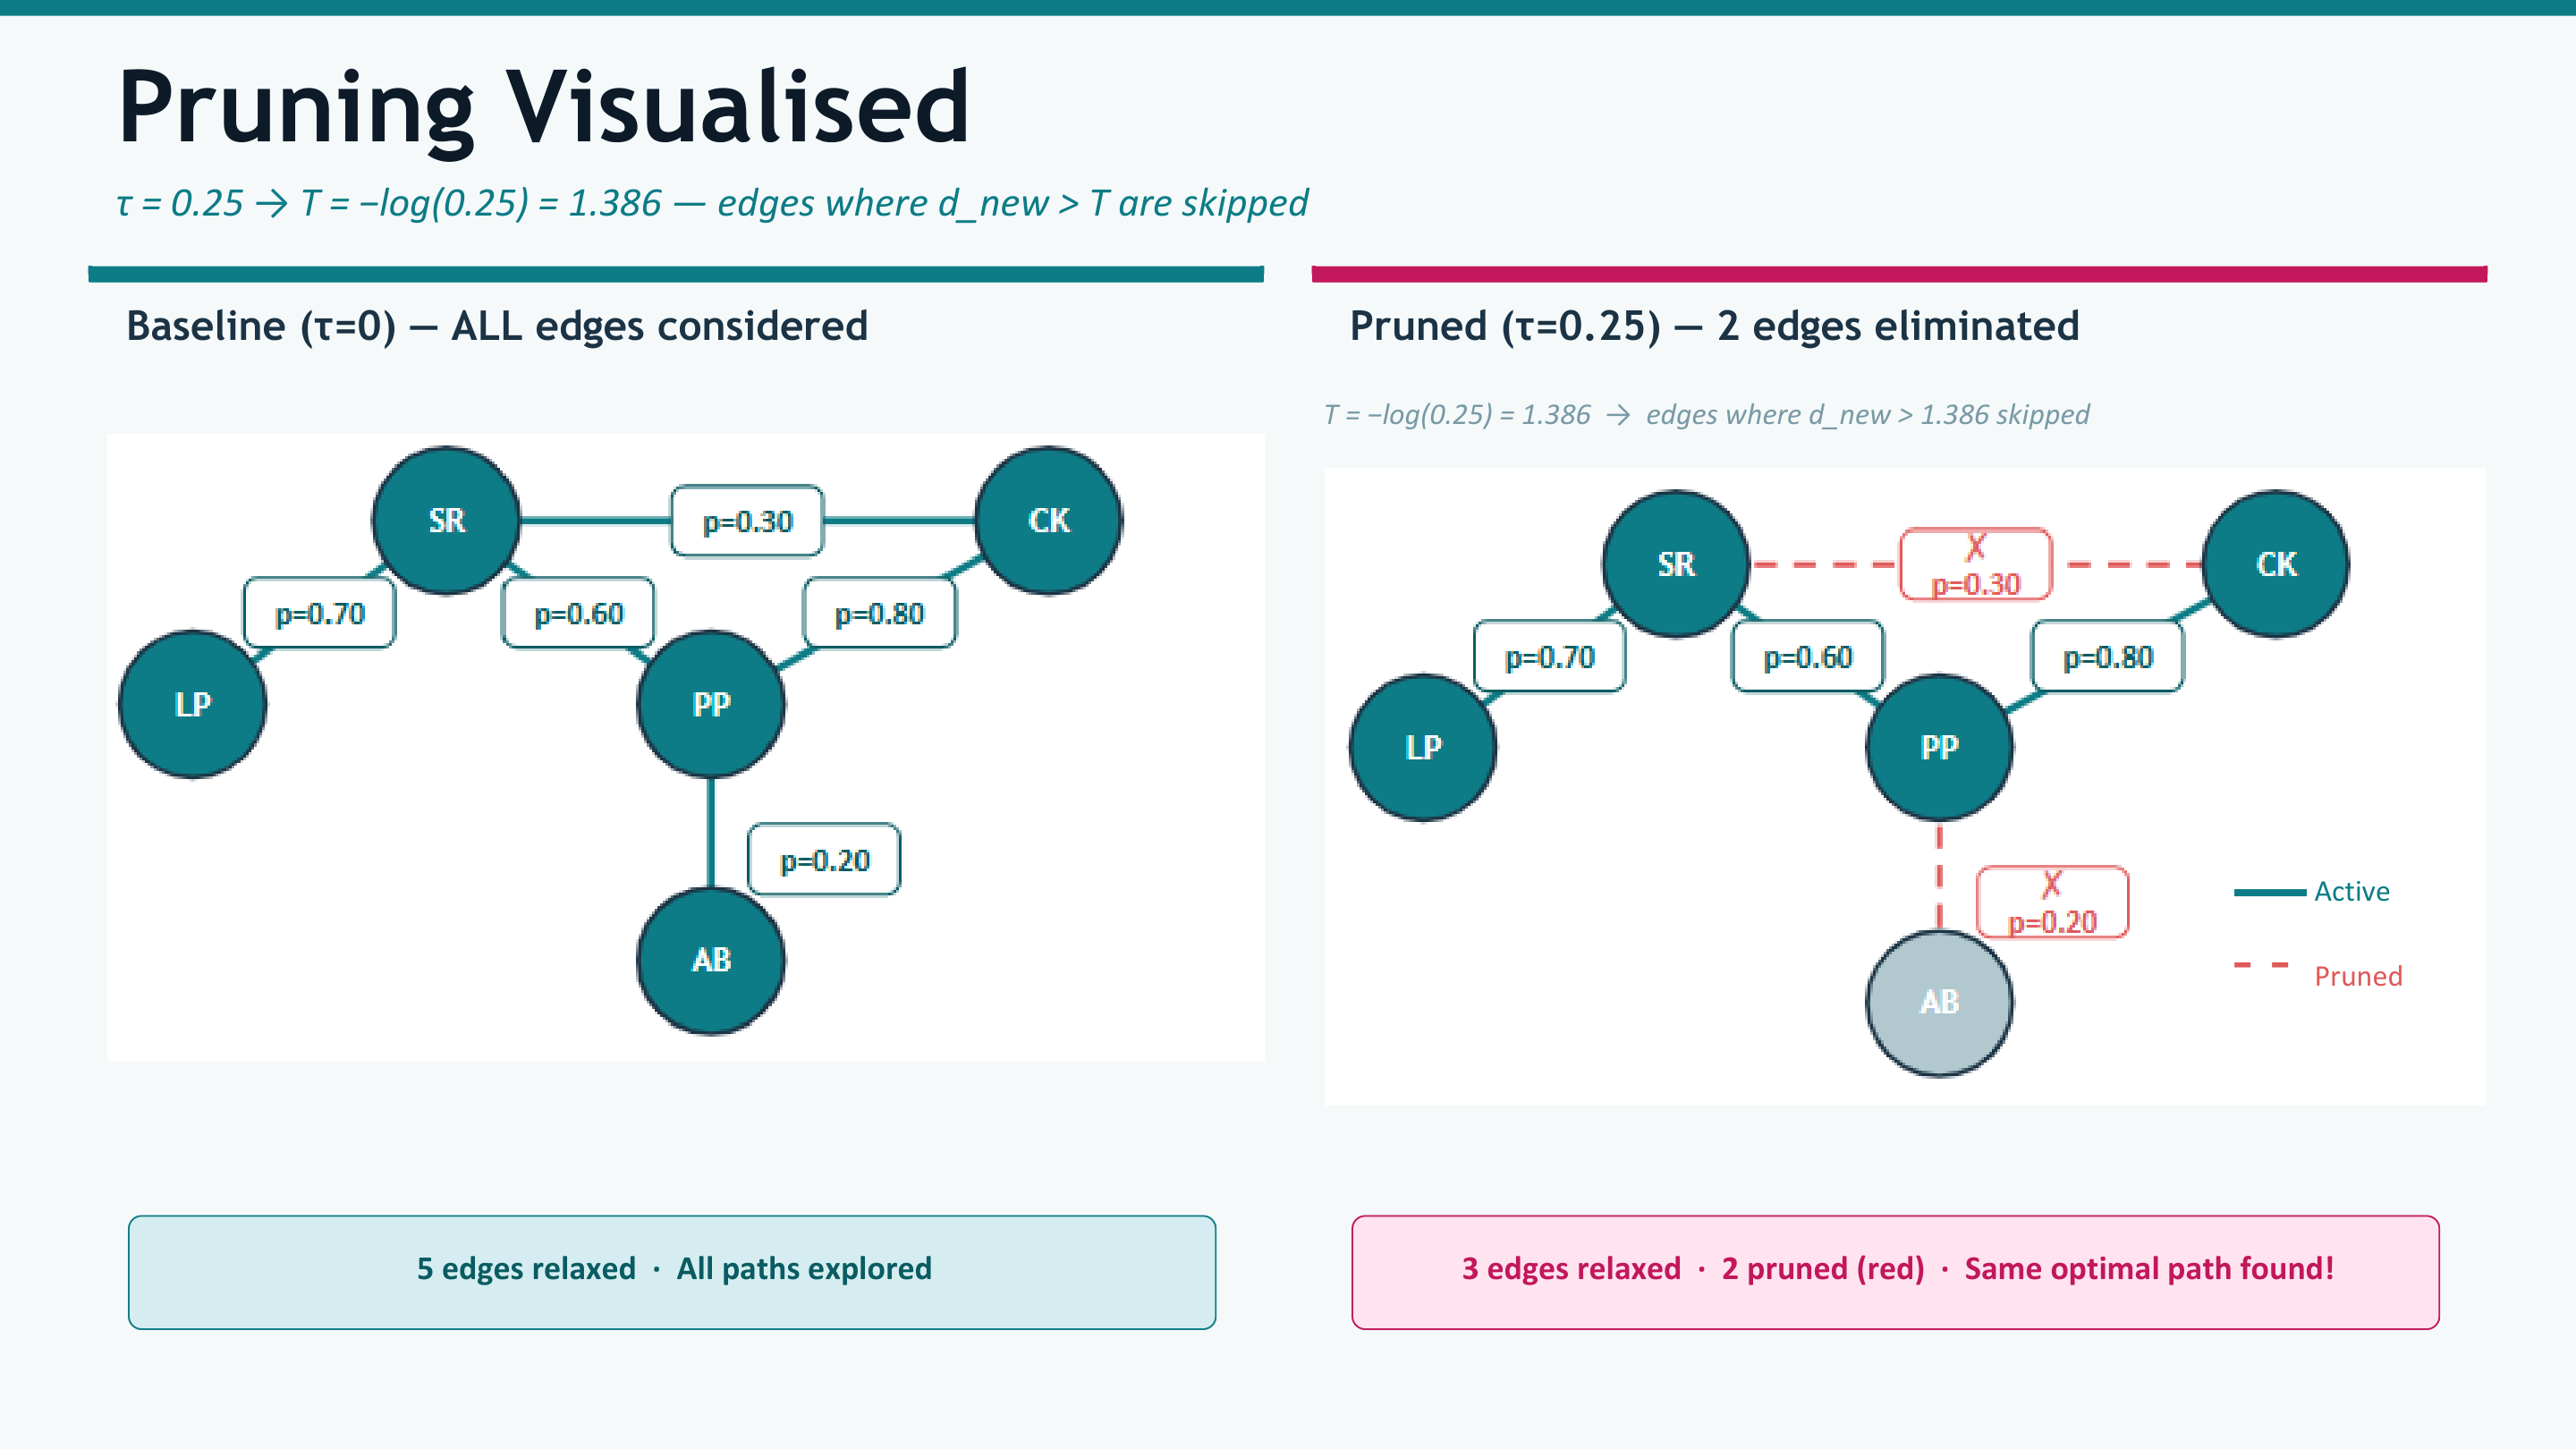
\includegraphics[width=0.92\textwidth]{pruning_visualised}
\caption[Pruning visualised: baseline vs.\ pruned Dijkstra on the example graph]{Pruning effect on the five-node customer journey graph with $\tau = 0.25$ ($T = -\log(0.25) = 1.386$). \textbf{Left:} Baseline Dijkstra relaxes all 5 edges. \textbf{Right:} Pruned Dijkstra eliminates 2 edges (dashed red) whose accumulated cost exceeds $T$---the SR$\to$CK shortcut and the PP$\to$AB branch---while still finding the same globally optimal path LP$\to$SR$\to$PP$\to$CK with only 3 edge relaxations.}
\label{fig:pruning_visualised}
\end{figure}

\subsection{Algorithm Comparison: Benefits and Drawbacks}
\label{sec:algocomparison}

Figure~\ref{fig:algo_flowchart} illustrates the decision-flow difference between both algorithms. In the baseline (left), every extracted node proceeds directly to neighbour relaxation. In the pruned variant (right), an extra threshold check $d_{\text{new}}>T=-\log(\tau)$ is inserted before each relaxation: edges exceeding the threshold are discarded (red PRUNE box), reducing the priority queue frontier and heap-operation overhead. Table~\ref{table:algo_compare} summarises the resulting trade-offs across eight criteria. The pruned algorithm will be compared against the baseline Dijkstra algorithm to measure runtime improvements and solution quality differences across all experimental configurations.

% ----------------------------------------------------------------
% FIGURE 3: Algorithm Comparison Flowchart
% ----------------------------------------------------------------
\begin{figure}[h!]
\centering
\begin{tikzpicture}[
    node distance=0.5cm and 1.6cm,
    startstop/.style={rectangle, rounded corners=8pt, minimum width=2.5cm, minimum height=0.7cm,
                      draw=black, thick, font=\small\bfseries, text centered},
    process/.style={rectangle, minimum width=2.5cm, minimum height=0.7cm,
                    draw=black, thick, font=\small, text centered},
    decision/.style={diamond, aspect=1.8, minimum width=2.8cm, minimum height=0.6cm,
                     draw=black, thick, font=\scriptsize\bfseries, text centered},
    prune/.style={rectangle, minimum width=2.5cm, minimum height=0.7cm,
                  draw=red!70!black, thick, fill=boxred, font=\small, text centered},
    arr/.style={-{Stealth[length=4pt]}, thick},
    lbl/.style={font=\scriptsize, fill=white, inner sep=1pt}
]

%--- LEFT COLUMN: Baseline Dijkstra ---
\node[startstop, fill=boxorange] (b_start) {Extract-Min$(Q)$};
\node[decision, below=0.5cm of b_start]  (b_tgt)   {$u = t$?};
\node[decision, below=0.7cm of b_tgt]    (b_stale)  {Stale?};
\node[process,  below=0.7cm of b_stale, fill=boxblue] (b_relax) {Relax neighbours};
\node[process,  below=0.5cm of b_relax, fill=boxblue] (b_push)  {Push to $Q$ if better};

% Straight-down arrows
\draw[arr] (b_start) -- (b_tgt);
\draw[arr] (b_tgt)   -- node[lbl,right]{No}  (b_stale);
\draw[arr] (b_stale) -- node[lbl,right]{No}  (b_relax);
\draw[arr] (b_relax) --                      (b_push);

% "Yes => Stop" from b_tgt:  go right, drop all the way to b_push level, merge in
\draw[arr] (b_tgt.east)
    -- ++(1.1,0)
    |- node[lbl, pos=0.25, right]{Yes $\Rightarrow$ \textbf{Stop}}
    (b_push.east);

% "Yes => Skip" from b_stale: go right, drop to b_relax level, merge in
\draw[arr] (b_stale.east)
    -- ++(0.8,0)
    |- node[lbl, pos=0.25, right]{Yes $\Rightarrow$ Skip}
    (b_relax.east);

\node[font=\small\bfseries, above=0.25cm of b_start, color=nodeorange] {Baseline Dijkstra};

%--- RIGHT COLUMN: Pruned Dijkstra ---
\node[startstop, fill=boxorange, right=3.8cm of b_start] (p_start) {Extract-Min$(Q)$};
\node[decision,  below=0.5cm of p_start]  (p_tgt)   {$u = t$?};
\node[decision,  below=0.7cm of p_tgt]    (p_stale)  {Stale?};
\node[decision,  below=0.7cm of p_stale]  (p_prune)  {$d_{\text{new}} > T$?};
\node[prune,     below=0.5cm of p_prune]  (p_skip)   {\textbf{PRUNE} (skip)};
\node[process,   right=1.3cm of p_prune, fill=boxblue] (p_relax)  {Relax edge};
\node[process,   below=0.5cm of p_skip,  fill=boxblue] (p_push)   {Push to $Q$ if better};

% Straight-down arrows
\draw[arr] (p_start) -- (p_tgt);
\draw[arr] (p_tgt)   -- node[lbl,right]{No}  (p_stale);
\draw[arr] (p_stale) -- node[lbl,right]{No}  (p_prune);
\draw[arr] (p_prune) -- node[lbl,left] {Yes} (p_skip);
\draw[arr] (p_skip)  --                      (p_push);

% "No" from p_prune goes right to p_relax, then p_relax drops down to p_push
\draw[arr] (p_prune.east) -- node[lbl,above]{No} (p_relax);
\draw[arr] (p_relax.south) |- (p_push.east);

% "Yes => Stop" from p_tgt: go right, drop all the way to p_push level
\draw[arr] (p_tgt.east)
    -- ++(1.4,0)
    |- node[lbl, pos=0.25, right]{Yes $\Rightarrow$ \textbf{Stop}}
    (p_push.east);

% "Yes => Skip" from p_stale: go right, drop to p_prune level
\draw[arr] (p_stale.east)
    -- ++(1.1,0)
    |- node[lbl, pos=0.25, right]{Yes $\Rightarrow$ Skip}
    (p_prune.east);

\node[font=\small\bfseries, above=0.25cm of p_start, color=nodegreen] {Pruned Dijkstra};
\end{tikzpicture}
\caption[Algorithm decision-flow comparison]{Decision-flow comparison of Baseline Dijkstra (left) and Pruned Dijkstra (right). The pruned variant adds a threshold check $d_{\text{new}}>T$ (red box); edges exceeding $T=-\log(\tau)$ are discarded without relaxation.}
\label{fig:algo_flowchart}
\end{figure}

\begin{table}[h!]
\centering
\renewcommand{\arraystretch}{1.3}
\begin{tabular}{@{}p{2.8cm}p{5.5cm}p{5.5cm}@{}}
\toprule
\textbf{Criterion} & \textbf{Baseline Dijkstra} & \textbf{Probability-Pruned Dijkstra} \\
\midrule
\textbf{Optimality} & Guaranteed globally optimal path for all $G$ with non-negative weights~\citep{dijkstra1959} & Guaranteed optimal only when $\tau = 0$; may return sub-optimal path for $\tau > 0$ \\[4pt]
\textbf{Time Complexity} & $O(|E|\log|V|)$ (worst and average case identical)~\citep{cormen2009} & $O(|E|\log|V|)$ worst case; $O(|E'|\log|V|)$ expected, $|E'| \leq |E|$ \\[4pt]
\textbf{Space Complexity} & $O(|V|+|E|)$ & $O(|V|+|E|)$ (unchanged) \\[4pt]
\textbf{Runtime on Large Graphs} & Can be slow on large, dense graphs due to full frontier expansion & Expected to be faster due to reduced frontier size and fewer heap operations \\[4pt]
\textbf{Parameter Tuning} & None required & Requires selection of $\tau$; too large risks missing optimal path \\[4pt]
\textbf{Approximation Bound} & Exact (no approximation) & No formal bound; trade-off evaluated empirically \\[4pt]
\textbf{Convergence} & Always finds optimal path if one exists & Converges to baseline as $\tau \to 0$~\citep{cormen2009} \\[4pt]
\textbf{Use Case} & Correctness-critical applications; small to medium graphs & Large graphs where approximation is acceptable; scalability-critical settings \\
\bottomrule
\end{tabular}
\caption[Algorithm comparison]{Comparison of Baseline and Pruned Dijkstra across key criteria. See Chapter~\ref{chap:complexity} for full complexity analysis.}
\label{table:algo_compare}
\end{table}

\section{Data Structures}

Figure~\ref{fig:data_structures} summarises the three complementary data structures used in both algorithms, along with their critical operation complexities. Each structure is chosen for a specific asymptotic property that directly contributes to the overall $O(|E|\log|V|)$ time bound.

\begin{figure}[h!]
\centering
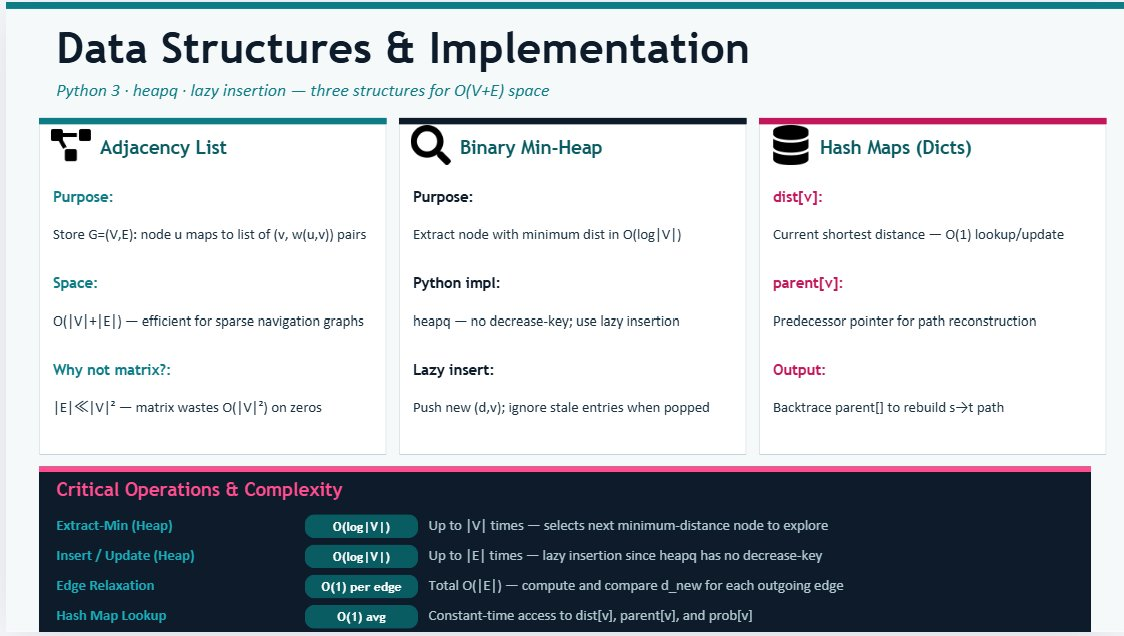
\includegraphics[width=0.95\textwidth]{data_structures}
\caption[Data structures and implementation overview]{Data structures and implementation overview for both algorithms. \textbf{Top row:} Adjacency List ($O(|V|+|E|)$ space, efficient for sparse graphs); Binary Min-Heap (Python \texttt{heapq} with lazy insertion, $O(\log|V|)$ extract-min and insert); Hash Maps (\texttt{dist[v]} and \texttt{parent[v]} with $O(1)$ average lookup). \textbf{Bottom panel:} Critical operation complexities --- Extract-Min $O(\log|V|)$; Insert/Update $O(\log|V|)$; Edge Relaxation $O(1)$ per edge; Hash Map Lookup $O(1)$ average.}
\label{fig:data_structures}
\end{figure}

\subsection{Adjacency List}

The directed graph will be stored as an adjacency list mapping each node $u$ to its outgoing neighbours and associated log-transformed weights. This ensures $O(|V|+|E|)$ space and efficient $O(\deg(u))$ neighbour iteration---both critical for sparse navigation graphs~\citep{cormen2009}.

\subsection{Binary Min-Heap (Priority Queue)}

A binary min-heap will serve as the priority queue, supporting~\citep{cormen2009,fredman1987fibonacci}:
\begin{itemize}
    \item \textbf{Extract-min:} $O(\log|V|)$, occurring up to $|V|$ times per run.
    \item \textbf{Insert:} $O(\log|V|)$, occurring up to $|E|$ times per run.
    \item \textbf{Edge Relaxation:} Computing updated log-distances and the pruning condition per edge; total cost $O(|E|)$ across the full traversal~\citep{cormen2009}.
    \item \textbf{Neighbour Iteration:} Iterating outgoing edges of each extracted node; total cost $O(|E|)$.
\end{itemize}

\subsection{Hash Maps (Dictionaries)}

Hash maps store \texttt{dist[v]} and \texttt{parent[v]} with $O(1)$ average-case access~\citep{cormen2009}.

\section{Complexity and Correctness}

Full complexity analysis is presented in Chapter~\ref{chap:complexity} and the correctness argument plan in Chapter~\ref{chap:correctness}. Briefly: both algorithms run in $O(|E|\log|V|)$ worst-case time and $O(|V|+|E|)$ space; the pruned algorithm reduces expected-case time to $O(|E'|\log|V|)$ with $|E'|\leq|E|$. Correctness of the baseline follows from the greedy invariant of Dijkstra's algorithm; the pruned variant converges to the baseline as $\tau\to 0$.

\section{Experimental Design}
\label{sec:expdesign}

\subsection{Simulation Environment}

All experiments will be implemented in Python using only standard libraries to ensure transparency of algorithmic implementation. Graphs will be represented using adjacency lists and priority queues will be implemented using Python's \texttt{heapq}. Runtime will be measured using \texttt{time.perf\_counter()} and memory usage tracked using \texttt{tracemalloc}. Each experiment configuration will be repeated at least 10 times with fixed random seeds to ensure reproducibility and fair comparison. Table~\ref{table:simenv} summarises the planned environment. Using only standard library components ensures that all algorithmic choices---data structures, timing, and memory profiling---are directly comparable across configurations without interference from third-party library overhead.

\begin{table}[h!]
\centering
\renewcommand{\arraystretch}{1.3}
\begin{tabular}{@{}ll@{}}
\toprule
\textbf{Component} & \textbf{Planned Specification} \\
\midrule
Programming Language & Python (standard library only) \\
Graph Representation & Adjacency list (\texttt{dict}) \\
Priority Queue & \texttt{heapq} (binary min-heap) \\
Runtime Measurement & \texttt{time.perf\_counter()} \\
Memory Measurement & \texttt{tracemalloc} peak allocation \\
Random Seeds & Fixed per configuration (for reproducibility) \\
Repetitions & $\geq 10$ runs per configuration \\
Graph Generator & Custom sparse graph generator (in-house) \\
\bottomrule
\end{tabular}
\caption[Planned simulation environment]{Planned simulation environment. All components use Python standard library only to ensure transparent, reproducible comparisons.}
\label{table:simenv}
\end{table}

\subsection{Evaluation Metrics}

Each experiment will record the following metrics across both algorithms and all input sizes:
\begin{itemize}
    \item \textbf{Execution Time (ms):} Wall-clock time measured with \texttt{time.perf\_counter()}.
    \item \textbf{Peak Memory Usage (MB):} Maximum resident memory during execution, measured with \texttt{tracemalloc}, capturing the practical space overhead of both algorithms across input sizes.
    \item \textbf{Nodes Explored:} Number of vertices extracted from the priority queue.
    \item \textbf{Edges Relaxed:} Total edge relaxation operations performed.
    \item \textbf{Path Probability $\Pi^*$:} Final cumulative probability $\prod_{(u,v)\in P^*} p(u,v)$.
    \item \textbf{Relative Optimality Gap:}
    \[
    \Delta = \frac{|\Pi^*_{\text{baseline}} - \Pi^*_{\text{proposed}}|}{\Pi^*_{\text{baseline}}} \times 100\%
    \]
    where $\Pi^*_{\text{baseline}}$ and $\Pi^*_{\text{proposed}}$ denote the path probabilities (scalar values in $[0,1]$) returned by the baseline and pruned algorithms respectively.
    \item \textbf{Max Frontier Size (MaxPQSize):} Maximum number of elements in the priority queue during execution.
\end{itemize}

\subsection{Experimental Parameters}

The following parameters will be varied systematically:
\begin{itemize}
    \item \textbf{Input Size $|V|$:} 1,000 (small), 5,000--10,000 (medium), up to 50,000 (large).
    \item \textbf{Edge Density:} Average out-degree $\bar{d} \in \{2, 5, 10\}$ edges per node.
    \item \textbf{Probability Distribution:} Uniform $\mathcal{U}(0,1]$ vs.\ skewed (power-law with exponent $\alpha = 2$).
    \item \textbf{Pruning Threshold $\tau$:} $\{0,\; 0.001,\; 0.01,\; 0.05,\; 0.1,\; 0.5\}$.

    \item \textbf{Graph Type:} Erd\H{o}s--R\'enyi sparse random graphs and layered/stage-based customer-journey graphs.
    
\end{itemize}



\subsection{Experimental Controls}

\begin{itemize}
    \item Both algorithms run on identical graph instances (same seed, same generated graph).
    \item Single-threaded execution on a dedicated machine to eliminate scheduling noise.
    \item Each configuration repeated $\geq 10$ times; mean and standard deviation reported.
    \item Memory measured independently per run using \texttt{tracemalloc.get\_traced\_memory()}.
\end{itemize}

\subsection{Risks and Fallback Plan}

Main technical risks: (1) over-aggressive pruning at high $\tau$ eliminating near-optimal paths; (2) dense graphs limiting pruning benefit; (3) uniform probability distributions offering little search-space reduction; (4) large graphs approaching RAM limits.

Should pruning provide minimal runtime or memory improvement, the project will pivot to a detailed scalability analysis of the baseline, conduct a threshold sensitivity study, and present comparative results identifying when pruning is and is not effective. The minimum acceptable outcome is a validated baseline implementation, formal complexity analysis, and an empirical baseline-vs-pruned comparison demonstrating correctness, scalability, and reproducibility.
